\documentclass[final,hyperref={pdfpagelabels=false}]{beamer}
\usepackage{grffile}
\mode<presentation>{\usetheme{I6pd2}}


%\usecolortheme[snowy]{owl} %Yo puse este tema que me gusta.


\usepackage{babel}
\usepackage[latin1]{inputenc}
\usepackage{amsmath,amsthm, amssymb, latexsym}
%\usefonttheme[onlymath]{serif}
\boldmath



% ------------ Imágenes ----------------------
%Global Background must be put in preamble
\graphicspath{{figures/}}
\usepackage{graphicx}
\usebackgroundtemplate%

%{%
%    
\includegraphics[width=\paperwidth,height=\paperheight]{fondo}%
%}

% -------------------------------------------

\usepackage[orientation=portrait,size=a0,scale=1,debug]{beamerposter}




% change list indention level
% \setdefaultleftmargin{3em}{}{}{}{}{}


%\usepackage{snapshot} % will write a .dep file with all dependencies, allows for easy bundling

\usepackage{array,booktabs,tabularx}
\newcolumntype{Z}{>{\centering\arraybackslash}X} % centered tabularx columns
\newcommand{\pphantom}{\textcolor{ta3aluminium}} % phantom introduces a vertical space in p formatted table columns??!!

\listfiles




%%%%%%%%%%%%%%%%%%%%%%%%%%%%%%%%%%%%%%%%%%%%%%%%%%%%%%%%%%%%%%%%%%%%%%%%%%%%%%%%%%%%%%%%%%%%%%%%%%%%

%TODO ponerlos en un archivo sty:) así puedes tener tu propia paleta de colores
%para todos tus archivos de LaTeX!

% custom colors
\definecolor{i6blue}{cmyk}{1,0.305,0,0.06}
\definecolor{i6bluedark}{rgb}{0.0156,0.2578,0.5625} 
\definecolor{i6colorscheme1}{HTML}{261F55}  % e.g. for block title purple
\definecolor{i6colorblockbg}{HTML}{FF69B4}  % hotpink
\definecolor{i6colorblockfg}{HTML}{0A080E}  %purple black
\definecolor{i6colorscheme2}{HTML}{000000}  % e.g. title in headline
\definecolor{i6colorscheme3}{HTML}{DFDFDF}  % e.g. for poster background, gris claro
\definecolor{i6colorscheme4}{HTML}{000000} 
\definecolor{i6colorschemeHeadline}{HTML}{4F4F4F}  % for headline bg
\definecolor{i6colorschemeFootline}{HTML}{100D09}  % for headline bg

% headline colors and fonts
\setbeamercolor{headline}{fg=white,bg=i6colorschemeHeadline}
\setbeamercolor{title in headline}{fg=white}
\setbeamercolor{author in headline}{fg=white}
\setbeamercolor{institute in headline}{fg=lightgray}
\setbeamercolor{logo in headline}{fg=black,bg=lightgray}
\setbeamercolor{separation line}{bg=i6colorscheme1}


% body colors and fonts
\setbeamercolor*{normal text}{fg=black,bg=i6colorscheme3}

% block environment
\setbeamercolor*{block body}{bg=white,fg=black}
\setbeamercolor*{block title}{fg=i6colorblockfg,bg=i6colorblockbg}
\setbeamerfont{block title}{size=\large,series=\bf}

% example environment
\setbeamercolor*{example title}{fg=white,bg=i6colorscheme1}

\setbeamercolor{alerted text}{fg=i6colorscheme1}

\setbeamertemplate{itemize items}[triangle]
\setbeamertemplate{navigation symbols}{}  % no navigation on a poster

%%%%%%%%%%%%%%%%%%%%%%%%%%%%%%%%%%%%%%%%%%%%%%%%%%%%%%%%%%%%%%%%%%%%%%%%%%%%%%%%%%%%%%%%%%%%%%%%%%%%




			%% Símbolos matemáticos
			\newcommand*{\QEDA}{\null\nobreak\hfill\ensuremath{\blacksquare}}%
			\newcommand*{\QEDB}{\null\nobreak\hfill\ensuremath{\square}}%
			\newcommand{\TODO}[1]{\textcolor{purple}{#1}}
			\newcommand*{\final}{\null\nobreak\hfill\ensuremath{\diamond}}
			\newcommand{\IR}{\mathbb{R}}
			\newcommand{\IC}{\mathbb{C}}
			\newcommand{\IN}{\mathbb{N}}
			\newcommand{\IZ}{\mathbb{Z}}
			\newcommand{\suma}[3]{\sum\limits_{#1}^{#2}#3} %Sumas y series
			\newcommand{\union}[3]{\bigcup\limits_{#1}^{#2}{#3}} %uniones
			\newcommand{\producto}[3]{\prod_{#1}^{#2}{#3}} %productos
			\newcommand{\limite}[2]{\lim\limits_{#1}{#2}} %límites
			\newcommand{\limsu}[2]{\lim\limits_{#1 \rightarrow \infty }#2_{#1}}
			%para límites de sucesiones
			\newcommand{\Om}{\Omega}
			\newcommand{\cali}[1]{\mathcal{#1}} %Letras caligráficas
			\newcommand{\cont}[2]{$\mathcal{C} [#1, #2]$}
			\newcommand{\integ}[3]{\int_{#1}^{#2}{#3}}
			\newcommand{\ldos}{\mathit{l}^{2}}



%%%%%%%%%%%%%%%%%%%%%%%%%%%%%%%%%%%%%%%%%%%%%%%%%%%%%%%%%%%%%%%%%%%%%%%%%%%%%%%%%%%%%%


%Datos de la portada
\setlogo{logo_BUAP}
%\setauthorurl{https://github.com/AmelieBernes/tesis-licenciatura}
\setauthoremail{ammel.bernes@gmail.com}
\setlugar{D\'ecimo Congreso Internacional de Matem\'aticas y sus Aplicaciones, CIMA 10}

\title{\huge Estudio y an\'alisis espectral de los polinomios discretos de Legendre}
\author{Am\'elie Bern\`es Carmona, Moises Soto Bajo y Javier Herrera Vega}
\institute[BUAP]{Benem\'erita Universidad Auton\'oma de Puebla}
\date[Sep. 8th, 2009]{Sep. 8th, 2009}


% -----------------------------------------  Bibliografía
\setbeamercolor{bibliography item}{parent=palette primary}
\usepackage[backend=bibtex,style=alphabetic]{biblatex}
\addbibresource{Referencias.bib}


%%%%%%%%%%%%%%%%%%%%%%%%%%%%%%%%%%%%%%%%%%%%%%%%%%%%%%%%%%%%%%%%%%%%%%%%%%%%%%%%%%%%%%
\newlength{\columnheight}
\setlength{\columnheight}{120cm}


%%%%%%%%%%%%%%%%%%%%%%%%%%%%%%%%%%%%%%%%%%%%%%%%%%%%%%%%%%%%%%%%%%%%%%%%%%%%%%%%%%%%%%
\begin{document}
\begin{frame}
  \begin{columns}
    % ---------------------------------------------------------%
    % Set up a column 
    \begin{column}{.49\textwidth}
      \begin{beamercolorbox}[center,wd=\textwidth]{postercolumn}
        %\begin{minipage}[T]{.95\textwidth}  % tweaks the width, makes a new \textwidth
         % \parbox[t][\columnheight]{\textwidth}{ % must be some better way to set the the height, width and textwidth simultaneously
            % Since all columns are the same length, it is all nice and tidy.  You have to get the height empirically
            % ---------------------------------------------------------%
            % fill each column with content  
                              
            \begin{block}{Motivaci\'on}
            Fijado un entero $n \geq 2$, representaremos se\~nales
            de dimensi\'on $n$ con vectores $x = (x_{m})_{m=0}^{n-1}$
            de $\IR^{n}$.
     
            Buscamos una base de $\IR^{n}$
            $$\cali{L}^{n} := \{ \cali{L}^{n,k} : \hspace{0.2cm} 0 \leq k \leq n-1 \}$$
              \begin{itemize}
              
             \item (\textcolor{i6colorblockbg}{Tama\~no}) 
			que sea ortonormal, pues as\'i se cumplir\'a que,
			para toda se\~nal $x \in \IR^{n}$, 
			\[
			x = \suma{k=0}{n-1}{\langle x, \cali{L}^{n,k} \rangle \cali{L}^{n,k}}
			\hspace{1cm} \textit{y} \hspace{1cm}
			||x||^{2} = \suma{k=0}{n-1}{\langle x, \cali{L}^{n,k} \rangle^{2}},
			\]
			y
	           
	        \item (\textcolor{i6colorblockbg}{Forma}) 
	        para la que sea posible establecer criterios
			sencillos sobre la forma de la gr\'afica  
			\[
			G_{x} := \{ (m, x_{m}): \hspace{0.2cm} 0 \leq m \leq n-1 \}
			\]			
			de $x$ en t\'erminos
			de la representaci\'on de esta respecto a la base $\cali{L}^{n}$.
               \end{itemize}
               
            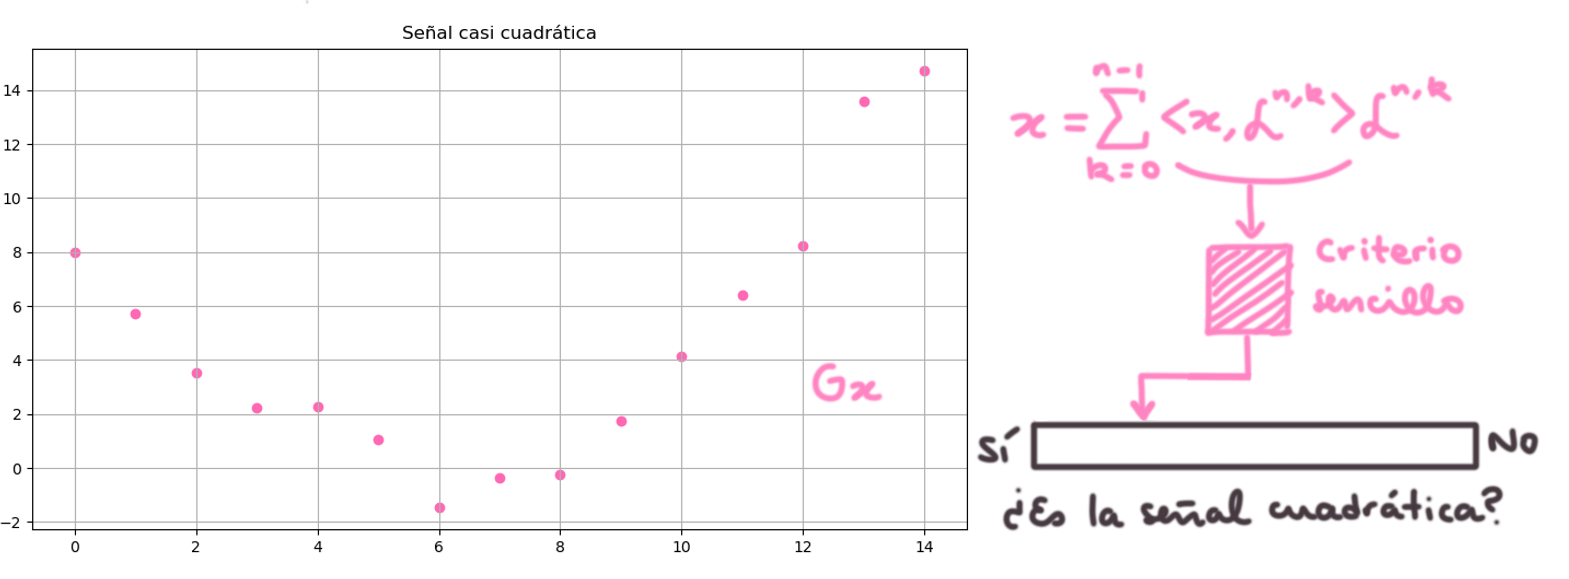
\includegraphics[width=0.95\linewidth]{cuadr2}
            \end{block}
            \vfill
		    \vspace{1cm}            
  
			\begin{block}{Construcci\'on}
			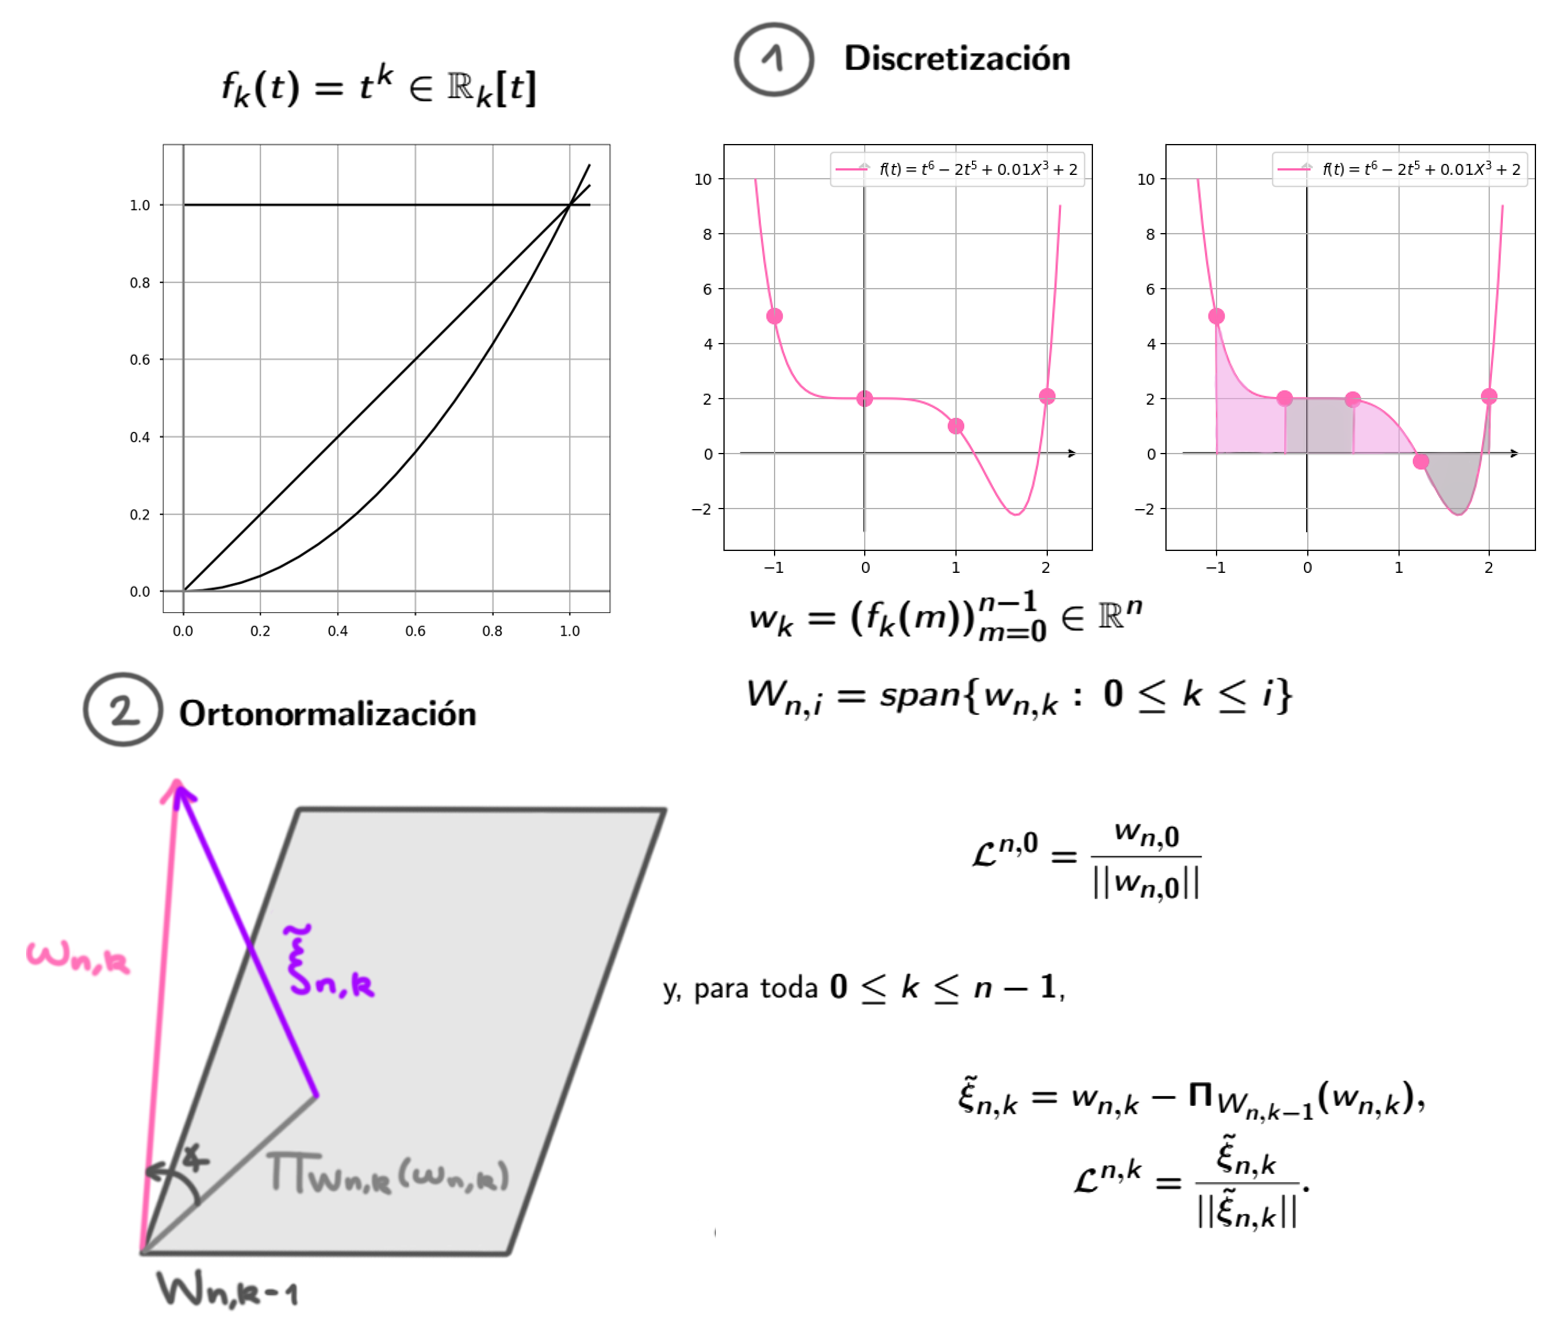
\includegraphics[width=0.95\linewidth]{esquema_construccion_bien}	
			Al vector $\cali{L}^{n,k} \in \IR^{n}$ se le llamar\'a el
			\textbf{polinomio discreto de Legendre de dimensi\'on $n$
			y grado $k$}, abreviado como PDL.
			\end{block}			                        
            \vfill
		    \vspace{1cm}
            
            
			\begin{block}{Espacios de polinomios discretos}
			\begin{center}
			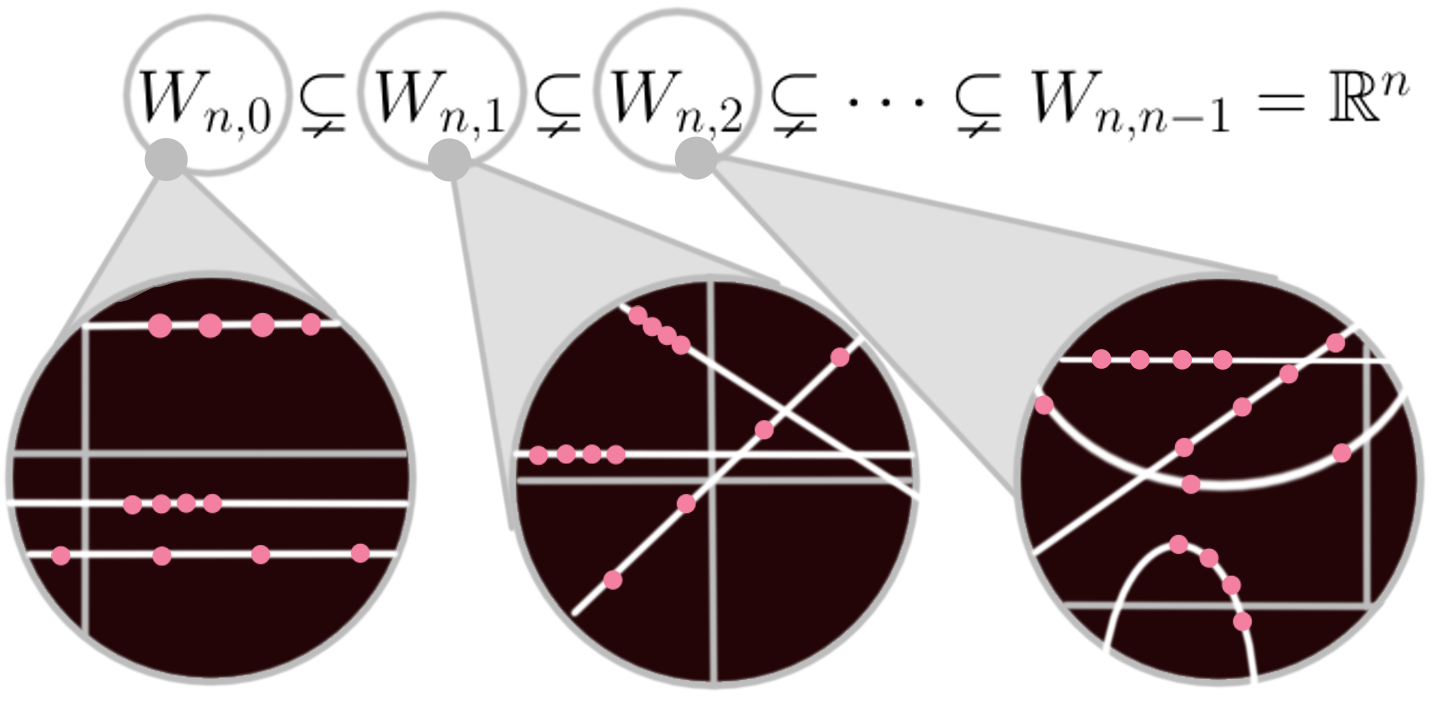
\includegraphics[width=0.7\linewidth]{nuevas_lupas}
			\end{center}
		
			\textbf{Noci\'on de grado para se\~nales $n-$dimensionales;}
			si $\cali{P}$ es una malla uniforme de $n$ puntos cualquiera,  
			\begin{itemize}
			\item el operador de discretizaci\'on puntual
			\[
			\Omega_{n, \cali{P}}: \IR_{n-1}[t] \longrightarrow \IR^{n}
			\]
			es un isomorfismo. Definimos el \textbf{grado de $x$}
			como el grado del \'unico polinomio $g \in \IR_{n-1}[t]$
			tal que $\Omega_{n, \cali{P}} (g) = x$ (se comprueba que esta
			definici\'on del grado no depende de la malla $\cali{P}$ fijada antes).
			\item Para toda se\~nal $x \in \IR^{n}$ y toda $0 \leq i \leq n-1$,
			$x \in W_{n, i}$ sii existe un polinomio $g(x)$ de grado a lo 
			m\'as $i$ tal que $x = \Omega_{n, \cali{P}}(g)$.
			\item Para toda $1 \leq i \leq n-1$, $x$ tiene grado $i$
			sii $x \in W_{n,i}$ pero $x \not\in W_{n, i-1}$.
			\end{itemize}
				
			\end{block}		
			\vfill	
			\vspace{1cm}
			
			
			\begin{block}{Referencias}
			\tiny{
			Charles P. Neuman y Dave I. Schonbach. "Discrete (Legendre) orthogonal
polynomials -a survey", International Journal for Numerical Methods in
Engineering: 8.4 (1974), p. 743-770 $\diamond$
Ranjan Roy. "The work of Chebyshev on orthogonal polynomials", Topics In 
Polynomials Of One And Several Variables And Their Applications: Volume
Dedicated to the Memory of P.L. Chebyshev $\diamond$
S.K. Suslov, V.B. Uvarov y Nikiforov A.F.  "Classical orthogonal polynomials
of a discrete variable". Springer Berlin Heidelberg (1991).}
			\end{block}
       
       
      \end{beamercolorbox}
    \end{column}
    % ---------------------------------------------------------%
    % end the column

    % ---------------------------------------------------------%
    % Set up a column 
    \begin{column}{.49\textwidth}
      %\begin{beamercolorbox}[center,wd=\textwidth]{postercolumn}
       % \begin{minipage}[T]{.95\textwidth} % tweaks the width, makes a new \textwidth
         % \parbox[t][\columnheight]{\textwidth}{ % must be some better way to set the the height, width and textwidth simultaneously
            % Since all columns are the same length, it is all nice and tidy.  You have to get the height empirically
            % ---------------------------------------------------------%

            	\begin{block}{Usando representaciones respecto a 
            	$\cali{L}^{n}$ para hacer an\'alisis de morfolog\'ia}
            	Se determina qu\'e tanto tiende una una se\~nal $x \in \IR^{n}$ a tener 
            	grado $k$ usando sus similitudes coseno a los espacios
            	$W_{n,k}$. Puesto que la forma de la gr\'afica de una se\~nal
            	es invariante ante multiplicaciones por escalares, note que
            	el usar similitudes coseno en vez de distancias euclideas es
            	mejor para dar una medida de la cercan\'ia de $x$ a un espacio
            	de polinomios discretos $n-$dimensionales.
			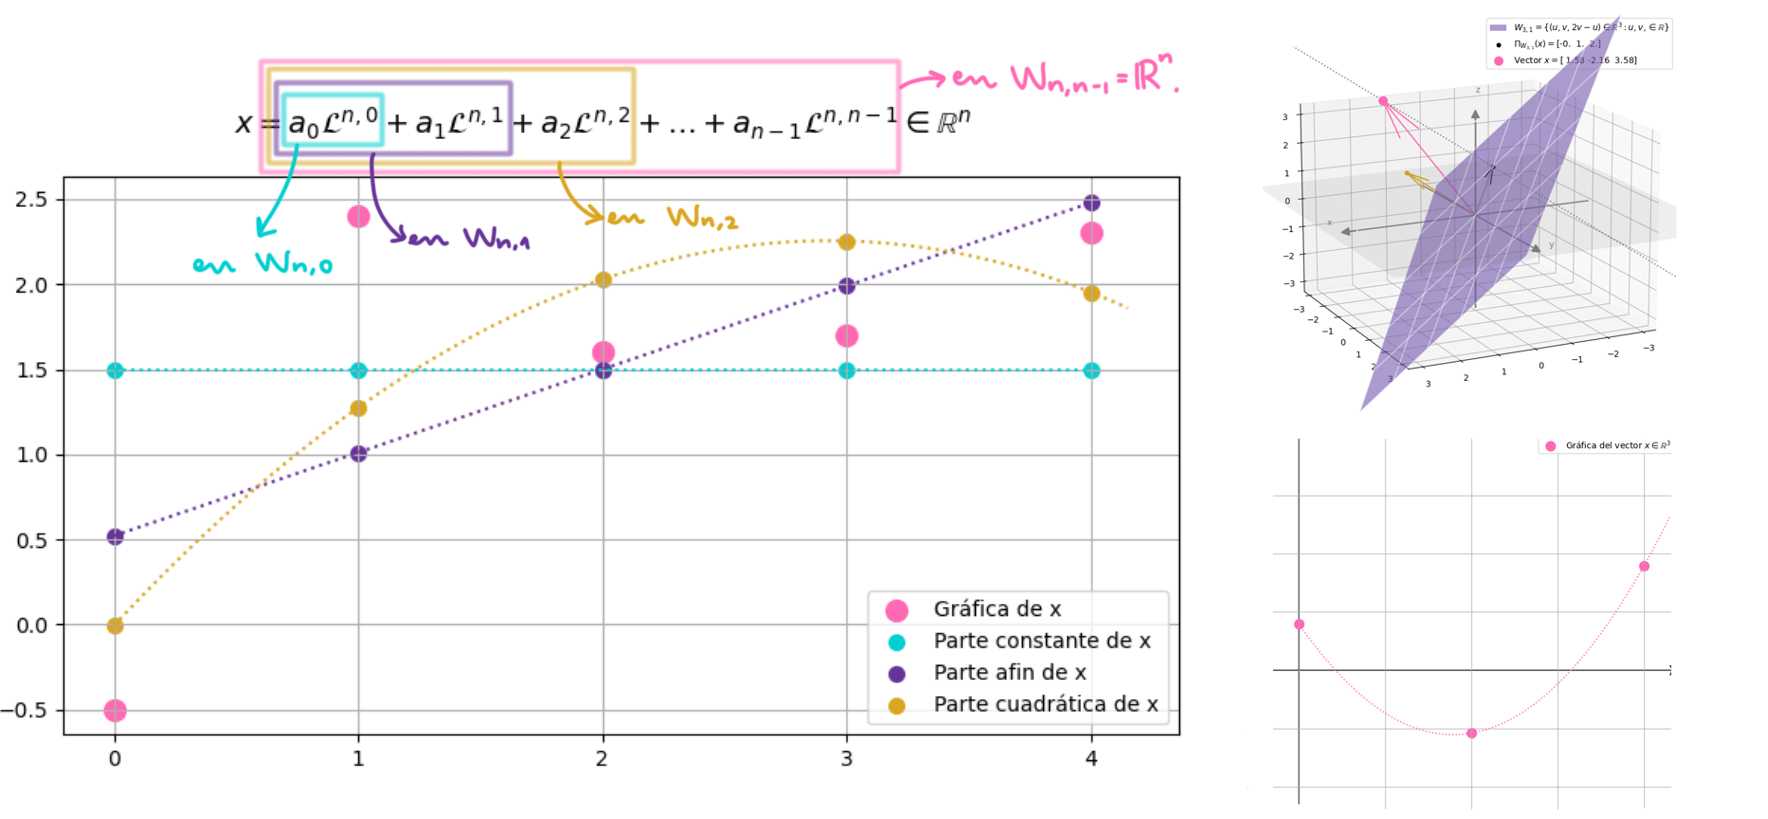
\includegraphics[width=0.95\linewidth]{analisis_forma}	
			Si $x \neq 0$ y $a_{i} := \langle x, \cali{L}^{n,i} \rangle$, entonces 
			\[
			cos(\measuredangle(x, W_{n,k})) = 			
			\frac{
			\sqrt{\suma{i=0}{k}{a_{i}^{2}}}}
			{\sqrt{\suma{i=0}{n-1}{a_{i}^{2}}}},
			\hspace{1.3cm} \textit{y} \hspace{1.3cm}
			x \in W_{n,k} \iff cos(\measuredangle(x, W_{n,k})) = 1.
			\]			
			\end{block}			                        
            \vfill
            \vspace{1cm}


            \begin{block}{An\'alisis espectrales de los PDL}
              \begin{columns}
                \begin{column}{.59\textwidth}
                  \vskip-3ex     
                  \begin{center}
                  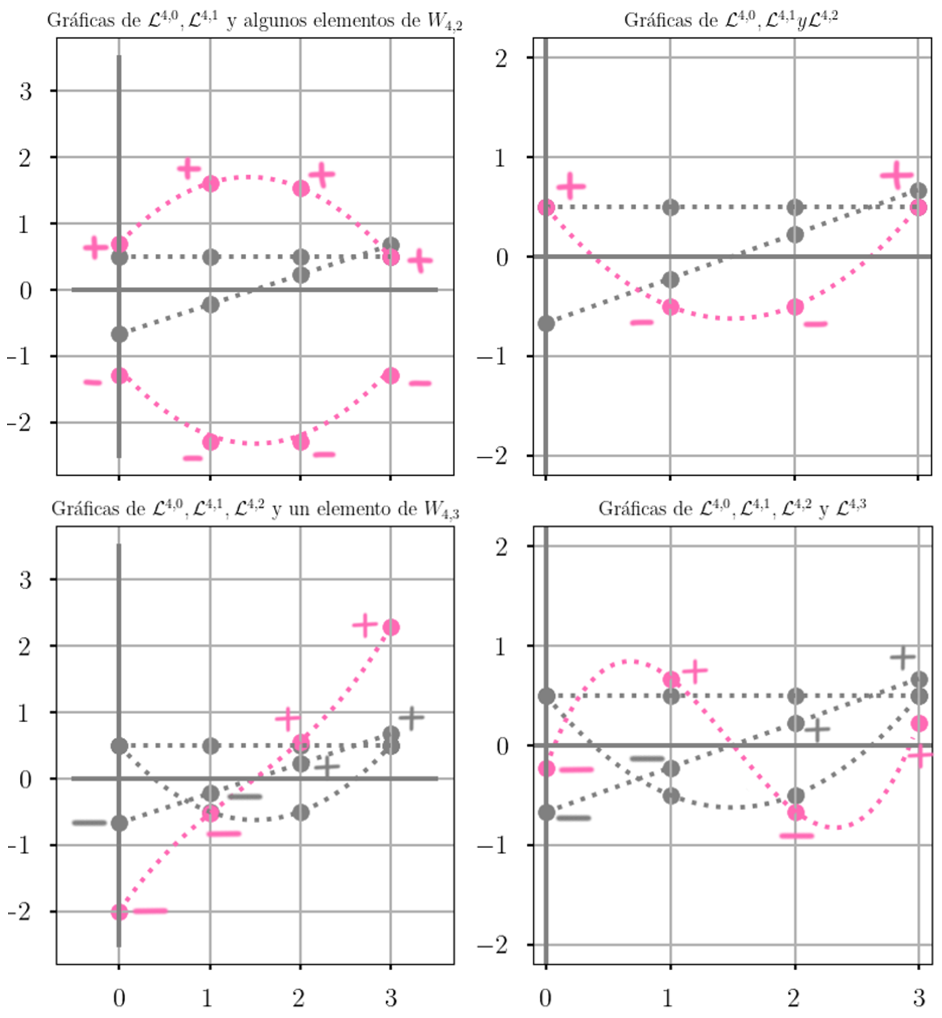
\includegraphics[width=0.4\linewidth]{oscil_motiv}
                  \end{center}
              	
              	Las condiciones de ortogonalidad en la definici\'on de los
              	PDL $\cali{L}^{n,k}$ 
              	implican un aumento en los cambios de signo de sus entradas
              	conforme la variable de grado $k$ aumenta.
                \end{column}
                \begin{column}{.39\textwidth}                
                  \vskip-3ex
                  Usando la transformada discreta de Fourier
                  \begin{center}
                   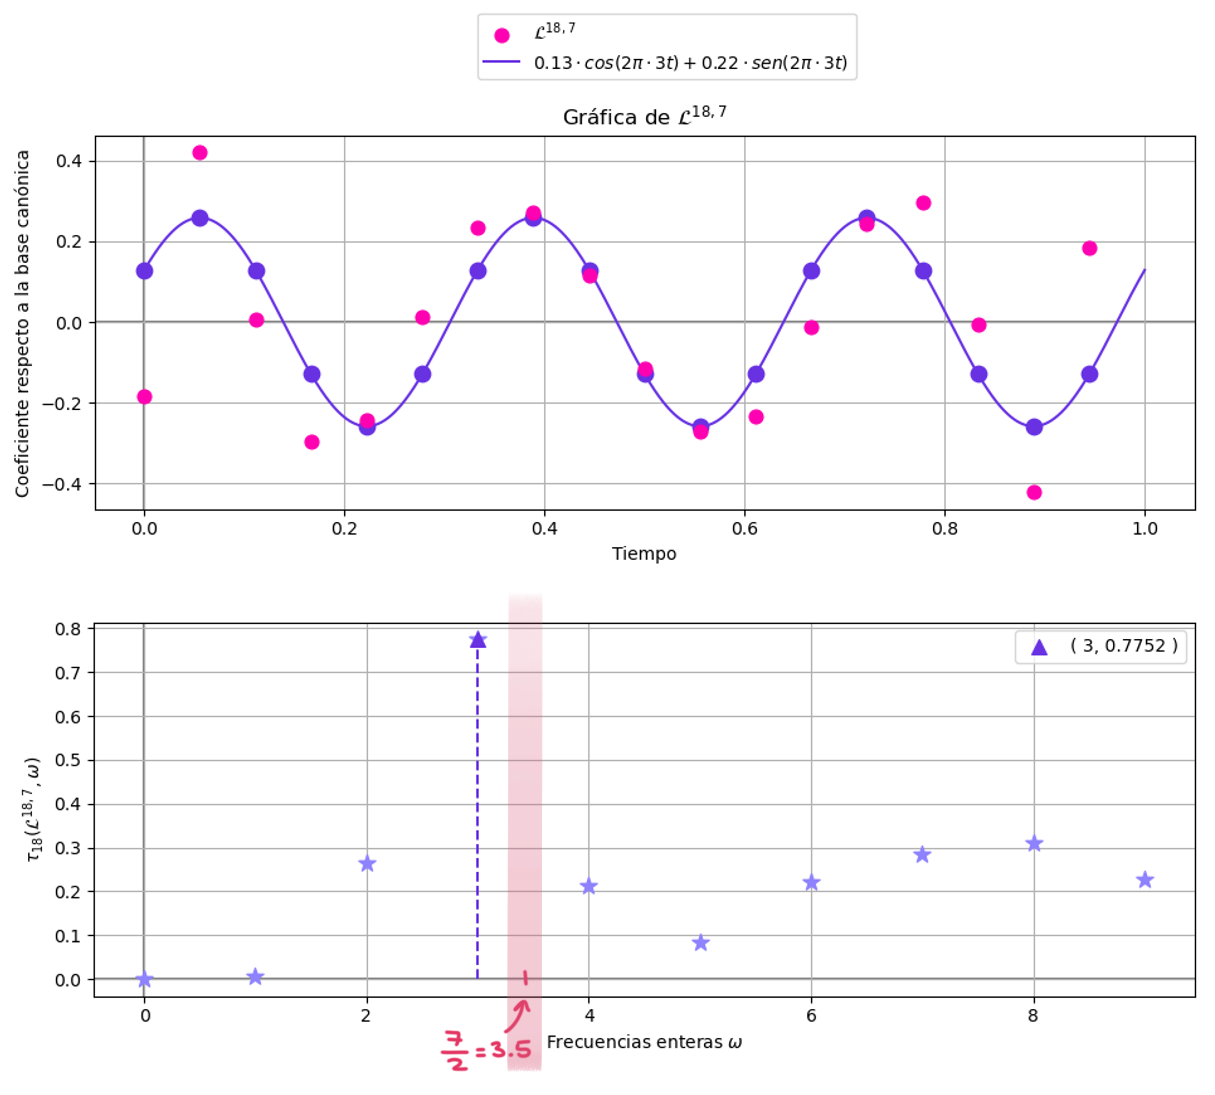
\includegraphics[width=0.7\linewidth]{espectroFourier_PDL_18_7}
                  \end{center}

                  Objetivo: poder tomar en consideraci\'on
                   frecuencias $\omega \geq 0$ arbitrarias.
                 
                \end{column}
              \end{columns}
            \end{block}
            \vfill
            \vspace{1cm}
            
            
            % ----------------------------------
            \begin{block}{An\'alisis espectral usando espacios monofrecuenciales}
              \begin{columns}
                \begin{column}{.59\textwidth}
                  \vskip-3ex     
                  Se\~nal $n-$dimensional de frecuencia pura $\omega$
				  $x = A \left( cos \left( 2 \pi \omega \frac{m}{n} + 
			      2 \pi \phi  \right) \right)_{m=0}^{n-1} \in \IR^{n}$. \\
              	
				\begin{center}
				Amplitud $A \geq 0$, frecuencia $\omega \geq 0$, desfase 
				$\phi \in [0,1[$.
				\end{center}				              	
              	Haciendo $A =1$ y $\phi = 0, \pi/2$ obtenemos los vectores
              	$c_{n, \omega}$ y $s_{n, \omega}$.
              	$x \in P_{n, \omega} := span \{ c_{n, \omega}, s_{n, \omega} \}$
              	sii $x$ es de frecuencia pura $\omega$. Si $x \neq 0$, definimos
              	\[
              	\sigma_{n, \omega} (x) =  cos(\measuredangle(x, P_{n, \omega})),
              	\]
              	y a su espectro $\Sigma_{x}: [0, n/2] \longrightarrow [0,1]$
              	como la funci\'on continua 
              	
              	\begin{align*}
\Sigma_{x}(\omega)= \begin{cases}
cos(\measuredangle(x, P_{n, \omega})) & 
\hspace{0.2cm} \textit{ si } \omega \in ]0, n/2[, \\
cos(\measuredangle(x, W_{n,1})) & \hspace{0.2cm} \textit{ si } \omega = 0, \\
cos(\measuredangle(A_{n}(x), W_{n,1})) & \hspace{0.2cm} \textit{ si } \omega = n/2.
\end{cases}
\end{align*}
              
                \end{column}
                \begin{column}{.39\textwidth}                
                  \vskip-3ex
                  Operador de alternancia $A_{n} : \IR^{n} \longrightarrow \IR^{n}$
                  \[
					\forall x = (x_{m})_{m=0}^{n-1} \in \IR^{n}:
			\hspace{0.5cm}
			A_{n}(x) = ((-1)^{m})_{m=0}^{n-1}.
			\]
                  \begin{center}
                   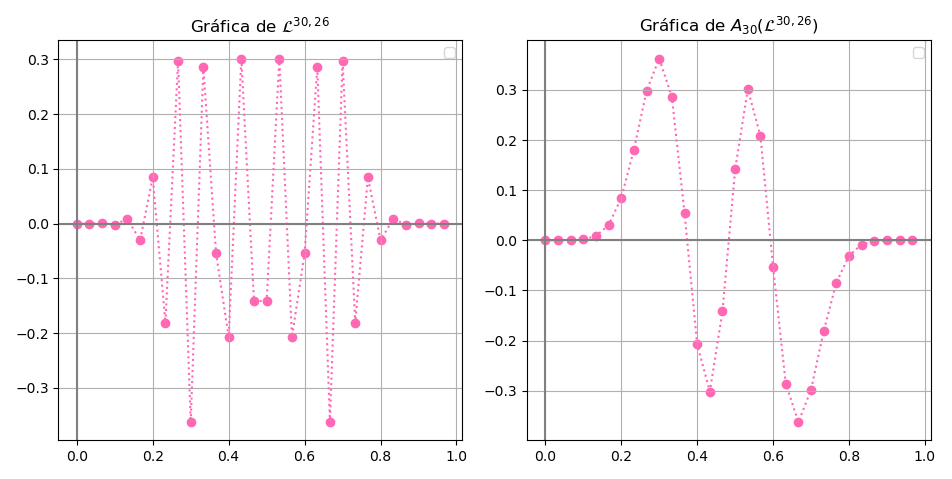
\includegraphics[width=0.6\linewidth]{alter_3}
                  \end{center}

				{\small{El espectro $\Sigma_{x}$ es una funci\'on
			\textbf{continua} y, exceptuando los puntos extremos, 
			\textbf{una extensi\'on
			del espectro de Fourier}.
				
					Para toda $0 < \omega < n/2$,
			entre m\'as cercano a uno sea $\Sigma_{x}(\omega)$,
			m\'as cerca estar\'a $x$ de tener la propiedad de ser
			de frecuencia pura $\omega$. A los $\omega \in [0, n/2]$
			en los que $\Sigma_{x}$ alcance su m\'aximo se les llamar\'a
			\textbf{frecuencias principales} de $x$.}}
%\vspace{1cm}
                \end{column}
              \end{columns}
              
              \begin{center}
                   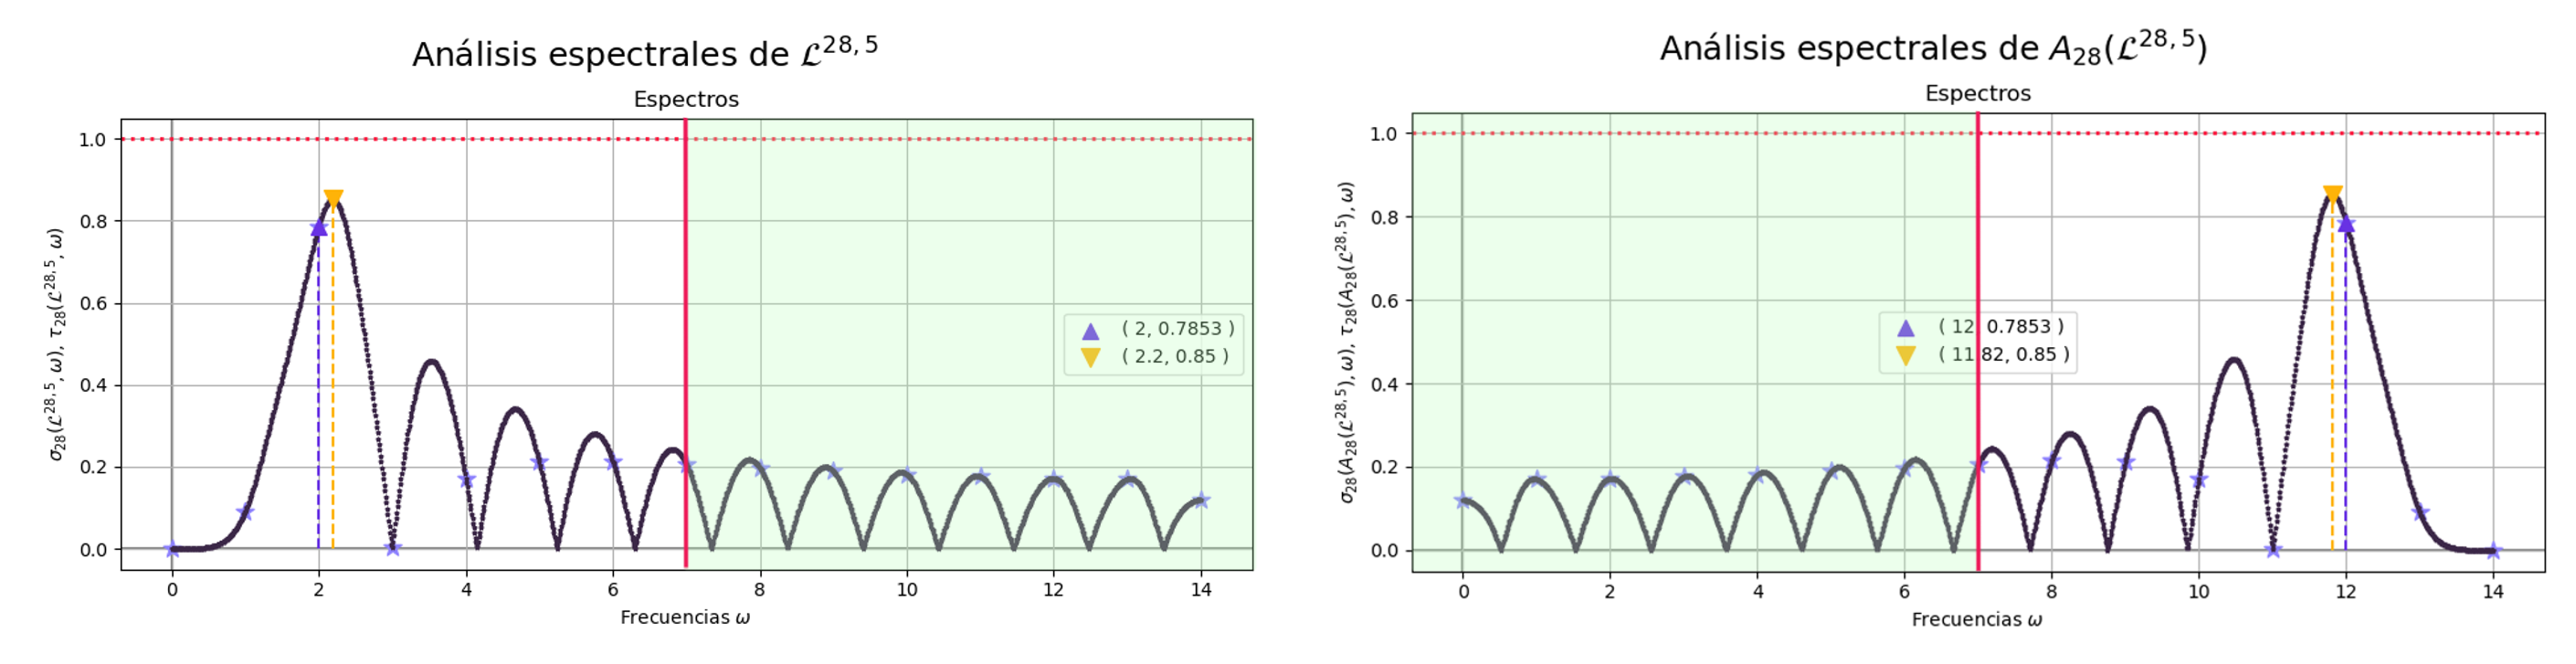
\includegraphics[width=0.7\linewidth]{alter_espec}
                  \end{center}
              
            \end{block}
            \vfill
            \vspace{1cm}
            
            

			%\begin{block}{Borrador}
			%Se\~nal $n-$dimensional de frecuencia pura $\omega$
			%$x = A \left( cos \left( 2 \pi \omega \frac{m}{n} + 
			%2 \pi \phi  \right) \right)_{m=0}^{n-1} \in \IR^{n}$ \\
			
			%$x \in P_{n, \omega} = span \{ c_{n, \omega}, s_{n, \omega} \}$ 		
			%si y s\'olo si $x$ tiene frecuencia pura $\omega$. \\
			
			%Si $x \neq 0$, 
			%\begin{align*}
			%\sigma_{n, \omega} (x) =  cos(\measuredangle(x, P_{n, \omega})) 
			%  \frac{||\Pi_{P_{n, \omega}}(x)||}{||x||}.
			%\end{align*}
			
			%Definimos el espectro de $x \in \IR^{n}-\{ 0 \}$ como la 
			%funci\'on continua 
			%$\Sigma_{x}: [0, n/2] \longrightarrow [0,1]$
			%dada por la expresi\'on
			
			%\begin{align*}
%\Sigma_{x}(\omega)= \begin{cases}
%cos(\measuredangle(x, P_{n, \omega})) & 
%\hspace{0.2cm} \textit{ si } \omega \in ]0, n/2[, \\
%cos(\measuredangle(x, W_{n,1})) & \hspace{0.2cm} \textit{ si } \omega = 0, \\
%cos(\measuredangle(A_{n}(x), W_{n,1})) & \hspace{0.2cm} \textit{ si } \omega = n/2.
%\end{cases}
%\end{align*}
			%\begin{itemize}
			%	\item Amplitud $A \in \IR$
			%	\item Frecuencia $\omega \geq 0$
			%	\item Desfase normalizado $\phi \in [0,1[$
			%\end{itemize}						
			
			%Operador de alternancia $A_{n}$
			%\[
			%\forall x = (x_{m})_{m=0}^{n-1} \in \IR^{n}:
			%\hspace{0.2cm}
			%A_{n}(x) = ((-1)^{m})_{m=0}^{n-1}.
			%\]			
			

                  %\begin{itemize}
			%\item El espectro $\Sigma_{x}$ as\'i definido es una funci\'on
			%continua y, exceptuando los puntos extremos, una extensi\'on
			%del espectro de Fourier.
			%\item Para toda $0 < \omega < n/2$,
			%entre m\'as cercano a uno sea $\Sigma_{x}(\omega)$,
			%m\'as cerca estar\'a $x$ de tener la propiedad de ser
			%de frecuencia pura $\omega$. A los $\omega \in [0, n/2]$
			%en los que $\Sigma_{x}$ alcance su m\'aximo se les llamar\'a
			%\textbf{frecuencias principales} de $x$.
			%\end{itemize}

			
			
			%\[
			%\cali{L}^{n, 0} = \frac{w_{n,0}}{||w_{n,0}||}
			%\]
			%y, para toda $0 \leq k \leq n-1$,
			%\[
			%\tilde{\xi}_{n,k} = w_{n, k} - \Pi_{W_{n, k-1}}(w_{n,k}),
			%\]
			%\[
			%\cali{L}^{n,k} = \frac{\tilde{\xi}_{n,k}}{||\tilde{\xi}_{n,k}||}.
			%\]
			
			%$w_{k} = \left( f_{k}(m) \right)_{m=0}^{n-1} \in \IR^{n}$		\\
			%$f_{k}(t) = t^{k} \in \IR_{k}[t]$ \\
			%$W_{n, i} = span \{ w_{n,k}: \hspace{0.2cm} 0 \leq k \leq i \}$
			
			%\textbf{Discretizaci\'on} \\
			%\textbf{Ortonormalizaci\'on}
			%\end{block}
			
			
			
         % }            
            
            
            \usebackgroundtemplate%


             \begin{block}{Conclusiones del an\'alisis espectral num\'erico}
             Parece ser que el valor $k/2$ es, m\'as que una estimaci\'on precisa de la
			frecuencia principal de un PDL de grado $k$, 
			una cota superior para tal frecuencia
			principal.
            En general, para todas las dimensiones $n$ estudiadas, se
		    encontr\'o que los PDL $\cali{L}^{n,k}$
			con $k$ peque\~no parec\'ian responder
			particularmente bien a su frecuencia principal, siendo el
			espectro evaluado en esta muy cercano a uno, pero conforme $n$
			crece y $k$ tiende a $n-1$ (su cota superior), los valores
			$\sigma_{n}(\cali{L}^{n,k}, \omega)$
			parecen estar muy alejados de $1$, por lo que no
			parece ser factible aproximar la gr\'afica de tales PDL
			s\'olo con un sinusoide.
			\begin{center}
				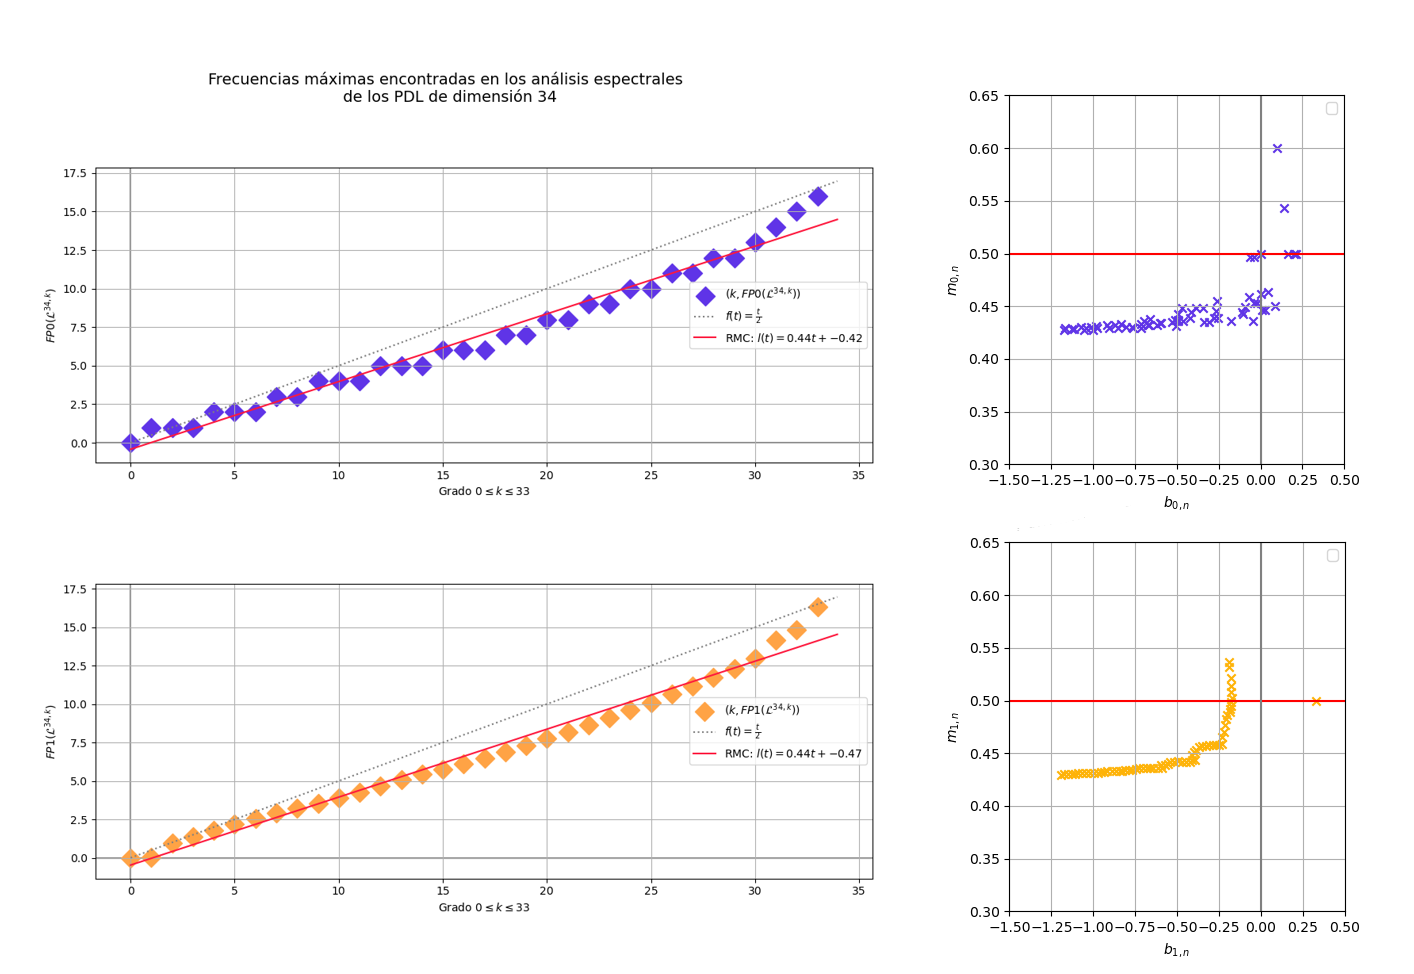
\includegraphics[width=0.6\linewidth]{resultados}
			\end{center}
			
			\end{block}			                    
            \vfill
            \vspace{1cm}
            

            
          %}
          % ---------------------------------------------------------%
          % end the column
        %\end{minipage}
      %\end{beamercolorbox}
    \end{column}
    % ---------------------------------------------------------%
    % end the column
  \end{columns}
  \vskip1ex
  %\tiny\hfill\textcolor{ta2gray}{Created with \LaTeX \texttt{beamerposter}  \url{http://www-i6.informatik.rwth-aachen.de/~dreuw/latexbeamerposter.php}}
\end{frame}
\end{document}

